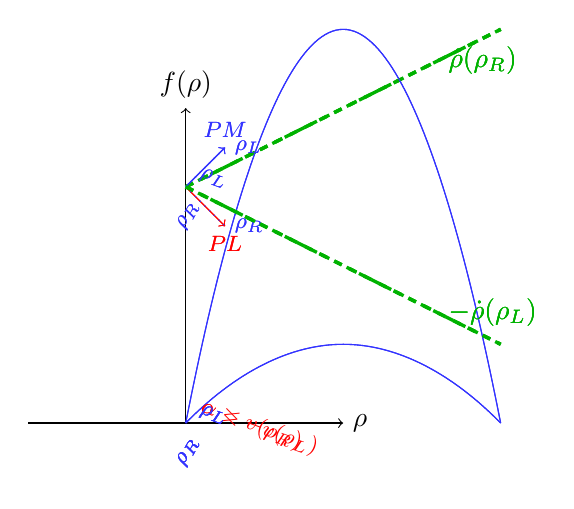
\begin{tikzpicture}[scale=1]
        % Axes
        \draw[->] (-2cm, -3cm) -- ++(4cm, 0cm) node[right] {$\rho$};
        \draw[->] (0cm, -3cm) -- ++(0cm, 4cm) node[above] {$f(\rho)$};

        % Initial states
        \draw[dashed, color=green!70!black, very thick] (0cm,0cm) -- (4cm,2cm) node[right, pos=.8] {$\dot{\rho}(\rho_R)$};
        \node[color=blue!80!white, anchor=south west, rotate=-20] at (0cm,0cm) {\footnotesize{$\rho_L$}};
        \node[color=blue!80!white, anchor=north east, rotate=60] at (0cm,0cm) {\footnotesize{$\rho_R$}};

        % Riemann solver for \rho > v(\rho_R)
        \draw[color=blue!80!white] (0cm,-3cm) parabola bend (2cm,2cm) (4cm,-3cm);
        \draw[color=blue!80!white] (0cm,-3cm) parabola bend (2cm,-2cm) (4cm,-3cm);
        \draw[color=green!70!black,very thick,dashed] (0cm,0cm) -- ++(4cm,2cm) node[right, pos=.8] {$\dot{\rho}(\rho_R)$};
        \draw[color=blue!80!white,->] (0cm,0cm) -- ++(.5cm, .5cm) node[above] {\footnotesize{$PM$}};
        \draw[color=red,->] (0cm,0cm) -- ++(.5cm, -.5cm) node[below] {\footnotesize{$PL$}};
        \draw[color=blue!80!white,dotted] (0cm,0cm) -- ++(.5cm, .5cm) node[right] {\footnotesize{$\rho_L$}};
        \draw[color=blue!80!white,dotted] (0cm,0cm) -- ++(.5cm, -.5cm) node[right] {\footnotesize{$\rho_R$}};
        \node[color=blue!80!white, anchor=south west, rotate=-20] at (0cm,-3cm) {\footnotesize{$\rho_L$}};
        \node[color=blue!80!white, anchor=north east, rotate=60] at (0cm,-3cm) {\footnotesize{$\rho_R$}};
        \draw[color=green!70!black, very thick, densely dashed] (0cm,0cm) -- ++(4cm,2cm) node[right, pos=.8] {$\dot{\rho}(\rho_R)$};
        \node[color=red, anchor=south west, rotate=-20] at (0cm,-3cm) {\footnotesize{$\alpha>v(\rho_R)$}};
        \node[color=blue!80!white, anchor=south west, rotate=-20] at (0cm,-3cm) {\footnotesize{$\rho_L$}};
        \node[color=blue!80!white, anchor=north east, rotate=60] at (0cm,-3cm) {\footnotesize{$\rho_R$}};

        % Initial states
        \draw[dashed, color=green!70!black, very thick] (0cm,0cm) -- (4cm,-2cm) node[right, pos=.8] {$-\dot{\rho}(\rho_L)$};
        \node[color=blue!80!white, anchor=south west, rotate=-20] at (0cm,0cm) {\footnotesize{$\rho_L$}};
        \node[color=blue!80!white, anchor=north east, rotate=60] at (0cm,0cm) {\footnotesize{$\rho_R$}};

        % Riemann solver for \rho > v(\rho_R)
        \draw[color=blue!80!white] (0cm,-3cm) parabola bend (2cm,-2cm) (4cm,-3cm);
        \draw[color=blue!80!white] (0cm,-3cm) parabola bend (2cm,2cm) (4cm,-3cm);
        \draw[color=green!70!black,very thick,dashed] (0cm,0cm) -- ++(4cm,-2cm) node[right, pos=.8] {$-\dot{\rho}(\rho_L)$};
        \draw[color=blue!80!white,->] (0cm,0cm) -- ++(.5cm, .5cm) node[above] {\footnotesize{$PM$}};
        \draw[color=red,->] (0cm,0cm) -- ++(.5cm, -.5cm) node[below] {\footnotesize{$PL$}};
        \draw[color=blue!80!white,dotted] (0cm,0cm) -- ++(.5cm, .5cm) node[right] {\footnotesize{$\rho_L$}};
        \draw[color=blue!80!white,dotted] (0cm,0cm) -- ++(.5cm, -.5cm) node[right] {\footnotesize{$\rho_R$}};
        \node[color=blue!80!white, anchor=south west, rotate=-20] at (0cm,-3cm) {\footnotesize{$\rho_L$}};
        \node[color=blue!80!white, anchor=north east, rotate=60] at (0cm,-3cm) {\footnotesize{$\rho_R$}};
        \draw[color=green!70!black, very thick, densely dashed] (0cm,0cm) -- ++(4cm,-2cm) node[right, pos=.8] {$-\dot{\rho}(\rho_L)$};
        \node[color=red, anchor=south west, rotate=-20] at (0cm,-3cm) {\footnotesize{$\alpha<-v(\rho_L)$}};
        \node[color=blue!80!white, anchor=south west, rotate=-20] at (0cm,-3cm) {\footnotesize{$\rho_L$}};
        \node[color=blue!80!white, anchor=north east, rotate=60] at (0cm,-3cm) {\footnotesize{$\rho_R$}};

    \end{tikzpicture}